\section{Technical Solution} \label{techsol}

The data pipeline for creating the visualizations has below important steps
as explained in \ref{fig:datapipeline}.

\begin{itemize}
\item Acquire the website usage data:
The scimaps.org uses the Webalizer tool \cite{weblizer}.
Webalizer
analyzes the web server logs to create HTML report which provide various
statistics of web site usage. While the actual web logs are available for
only 2016 the Weblizer HTML reports are available for last 10 years(March
2017 to February 2017). We used these Weblizer HTML reports as source. The
details of Weblizer reports, the exact HTML format and statistics captured is
 explained in the section \ref{sourcedata}.

\item Combine the data in single data store which can be queried:
Since the Weblizer HTML reports does not allow us to query the data, we
required to convert them into a structured format. We decided to convert the
HTML reports into comma-separated format (CSV). The section \ref{dataparser}
explains the implementation of the parser program which converts data into
CSV format. While designing the CSV format, we added metadata fields like
year and month so that we can filter the data for a specific duration.

\item Upload the data in visualization tool:
We used Tableau \cite{tableau} as our visualization tool for the
visualizations. Tableau supports importing CSV data.
\item Create individual visualizations:
We created multiple reports in Tableau to satisfy various project
requirements. Each Tableau report tries to answer a group of requirements for
 the project. Each report follows a similar pattern of filtering the data so
 as to maintain consistency across all reports. \ref{viz} section explains
 each visualization in detail.
\item Create a single storyboard by combining all visualizations:
While it is useful to analyze each dataset separately, it also helps to get a
 combined view of the overall website usage. We created storyboard from all
 the visualizations which helps in analyzing all the website usage data in
 one go. The storyboard provides interactive filters using which user can
 slice and dice data and analyze the usage pattern effectively.
\end{itemize}

\begin{figure}
\centering
\fbox{
\includegraphics[width=\linewidth]{img/datapipeline.png}}
\caption{Data Pipeline.}
\label{fig:datapipeline}
\end{figure}


\subsection{Source Data} \label{sourcedata}
\begin{figure}
\centering
\fbox{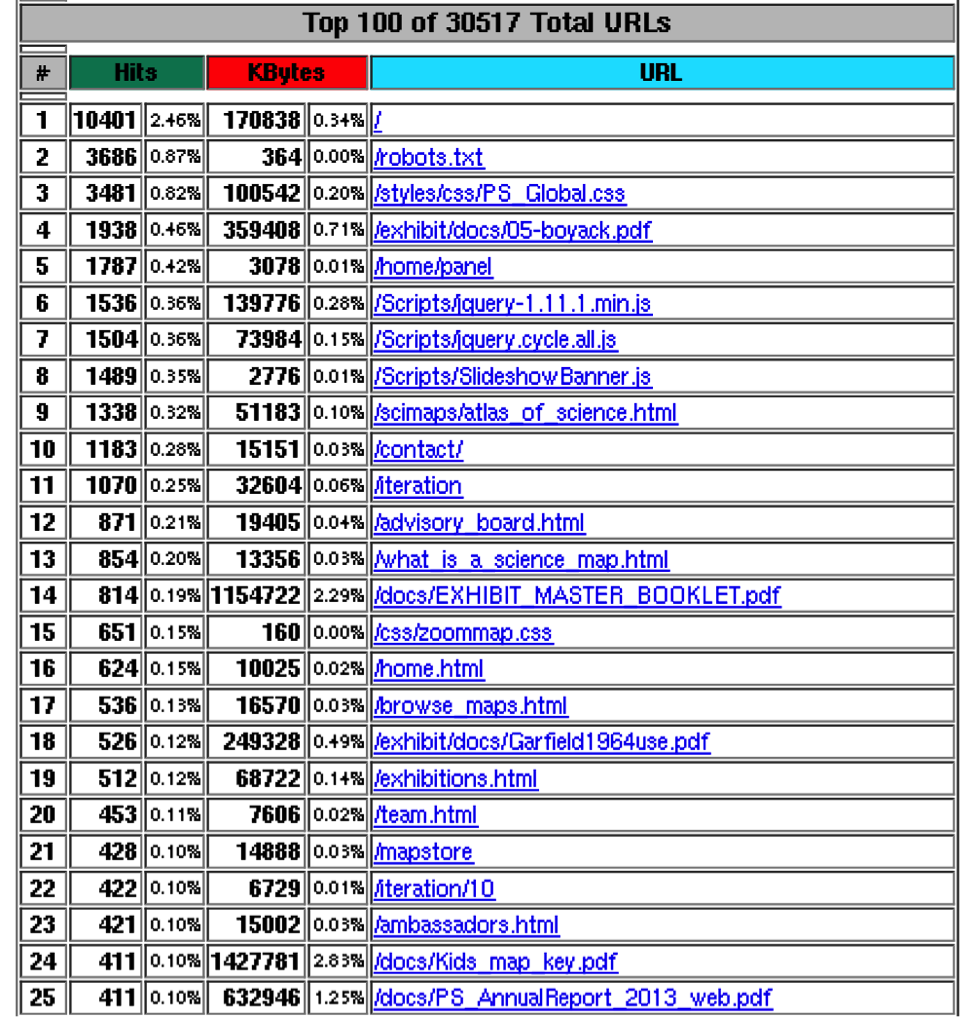
\includegraphics[width=\linewidth]{img/samplewebanalyzerreport.png}}
\caption{Sample Webanalyzer Report.}
\label{fig:samplewebanalyzer}
\end{figure}

As explained in section \ref{techsol}, the Webanalyzer reports in HTML format
are used as source data. These reports are available for last 10 years on
monthly basis. Each report has following sub-sections:
Monthly statistics, Daily statistics, Hourly statistics
, Top 100 URLs, Top 10 entry pages, Top 10 exit pages, Top 30 referring Sites, Top 20 search strings, Top 15 user agents, Top 10 countries

 Each section in webanalyzer report has HTML table. Figure
 \ref{fig:samplewebanalyzer} explains sample table from webanalyzer HTML
 report.


\subsection{Data Parser} \label{dataparser}
As explained in section \ref{techsol}, each Webanayzer HTML reports is
converted into CSV format. We implemented Data Parser Python script which
scrapes the
Webanalyzer HTML report and converts it into CSV structure. The data parser
uses Python module called BeautifulSoup to parse the HTML. It then iterates
over all 'A' tags to find the section header within HTML report. Finally it
iterates over the HTML table elements consisting TR and TD tags to extract
the data and writes it in CSV file.
 The data parser code is available at \cite{dataparser} repository. The
 figure \ref{fig:daystats} shows sample records from the DAYSTATS.csv which
 is one of the output CSV created by the data parser.

 \begin{figure}
\centering
\fbox{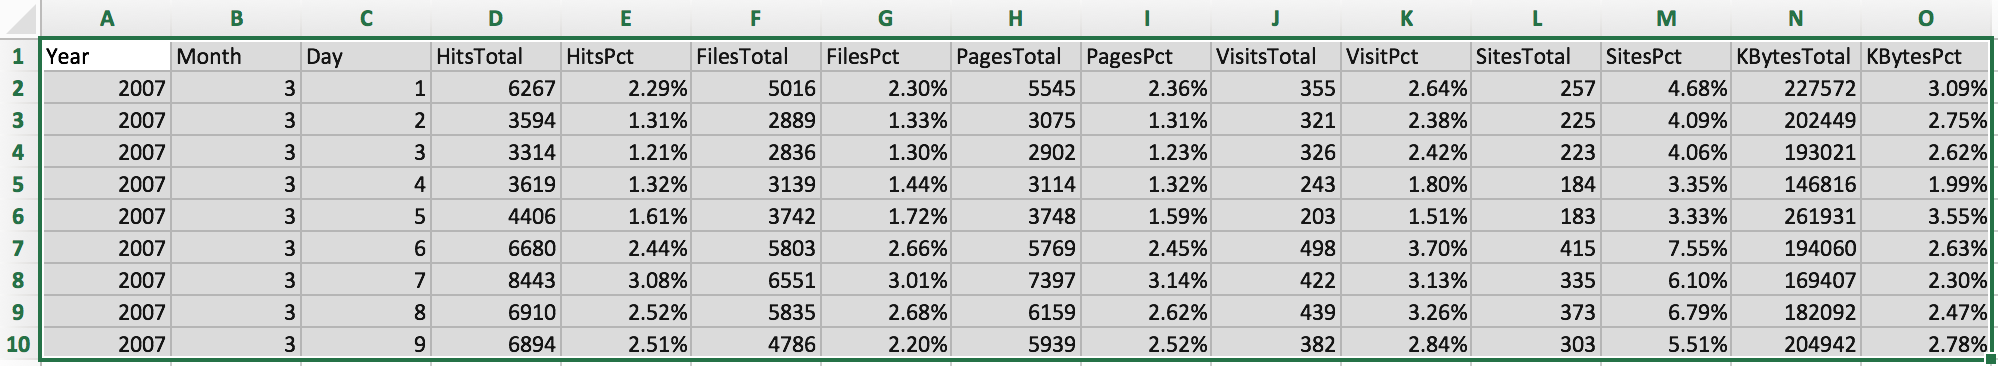
\includegraphics[width=\linewidth]{img/dailystats.png}}
\caption{Daily Statistics Sample Records.}
\label{fig:daystats}
\end{figure}




